\section{Experimental Setup}
\label{sec:exp-setup}

This section contains a description of both the data and the experiments that were conducted. The entirety of the code, alongside unannotated and annotated data, is provided in \autoref{app-resources}. The results of the experiments are presented and discussed in \autoref{sec:results}. A description of the data and the annotation process is provided in \autoref{subsec:data} and \autoref{subsec:annotation}. Generally, the experiments can be divided into three categories: tagger and lemmatizer testing (\autoref{subsec:bert-tagging}, \autoref{subsec:marmot-tagging}, \autoref{subsec:stanza-tagging}, \autoref{subsec:morfeusz-tagging}, \autoref{subsec:ud-tagging}, with the error analysis detailed in \autoref{subsec:error-annotation}), n-gram statistics (\autoref{subsec:ngrams}), and investigations into the National Corpus of Polish (\autoref{subsec:nkjp-vocab}). 

\subsection{Data}
\label{subsec:data}

The data used in the experiments originates from a memoir penned by Juliusz Czermiński in 1899 in Rzeszów. The original manuscript is preserved in the collection of Zakład Narodowy im. Ossolińskich (also known as Ossolineum) with the signature 15374/II, according to the library's catalog, but cannot be accessed digitally \citep{ossolineum}. At some point in the past, typewriter copies of the manuscript (possibly made from another copy and not the original manuscript) have been made and distributed among the author's descendants. In recent years, one of them, Piotr Kociat\-kiewicz, undertook the effort of copying over the text into a Word file, and it is this digitalized data that was used throughout the thesis. Unfortunately, due to the time constraints and the physical difficulty of accessing the manuscripts, no assessment of the quality of the transcription could be made.

As mentioned before, the data originates from one author and belongs to the genre of memoir. The author was a native of an area that encompasses nowadays south-eastern Poland and western Ukraine but was not independent at that time, and instead a part of the Austro-Hungarian Empire following the partitions of the Polish–Lithuanian Commonwealth in the late 18\textsuperscript{th} century. From what can be gathered from the contents of the memoir, the author considered himself to be Polish and wrote in an idiolect closely resembling the Polish language. However, due to the text's age and region of origin, it is likely that it diverges from standard modern Polish with regard to spelling (from which pronunciation may be inferred), grammar, and vocabulary. This assumption is strengthened by the fact that following the periodization of the history of Polish as outlined by \citet{długosz-kurczabowa_dubisz_2006}, the text could be classified as an example of writing in "early" New Polish (npol. 1.), which diverges from Modern or "late" New Polish (npol. 2.).
%% maybe this should be written elsewhere? but where?
%% add stuff from the other book once I unpack it

Both the relative understandability of the text to a native speaker of Polish and the potential for it to differ from standard Polish make it a good candidate for inquiries into how potential differences between a historical text and a modern standard could be identified computationally. It is, nevertheless, worth keeping in mind that this text need not be representative of Polish in general at the time of its writing and this thesis should be regarded as an investigation of this particular memoir and its author's language, not of late 19\textsuperscript{th} century Polish at large.

The entirety of the memoir consists of 37 405 tokens, according to Microsoft Word's word count functionality. Out of those, the first 360 sentences, corresponding to 10 286 tokens, were manually annotated with UPOS (universal part of speech) tags, and the first 115 sentences, corresponding to 3271 tokens, were additionally annotated with XPOS (language-specific part of speech) tags and lemmas following the tagsets used by \citet{wroblewska-2018-extended} in PDB (Polish Dependency Bank), which itself is the largest UD corpus available for Polish, and therefore conforms to the UD format. This decision was made due to the accessibility and universality of these tagsets, and because the results could then be compared to PDB's test set; additionally, some other tools, while not trained on PDB, seemed to be using the same tagset. The details of the annotation process are discussed in \autoref{subsec:annotation}. While this means that only roughly more than a quarter of the text was annotated with the UPOS tags and less than a tenth with the XPOS tags and lemmas, the annotation of the entire text was deemed to be beyond the scope of this thesis, especially given the complicated nature of the XPOS tags and the fact that the annotation had to be of high quality. Additionally, small test samples are not unheard of when it comes to tagger-related experiments using historical data \citep{bollmann-2013-pos, hupkes16, rayson07}. 

\begin{figure}[h]
\centering
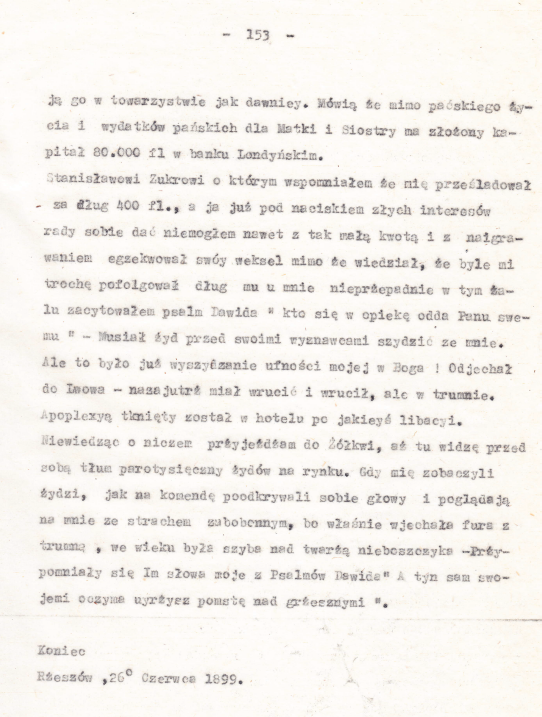
\includegraphics[scale=0.8]{memoir}
\caption{\label{fig:memoir} The final page of the typewriter transcription of the original text of the memoir, from which the digital copy was made. Private collection. Image courtesy of Anna Chodorowska.}
\end{figure}

Simultaneously, most of the procedures described in the subsequent subsections were also conducted on the PDB (Polish Dependency Bank) corpus, so that the results could be compared to those obtained on modern data; additionally, some of the taggers were locally trained on the PDB train set. As mentioned before, PDB is the largest UD-style treebank available for Polish. It features 22 152 sentences consisting of a total of 347 377 tokens, annotated according to the UD guidelines in the CoNLL-U format. Aside from the lemmas, UPOS, and XPOS tags, which are utilized in this project, the treebank also features an annotation of syntactic relations between words \citep{wroblewska-2018-extended, universaldependencies}.

Another corpus utilized in this thesis is the National Corpus of Polish, a large collection of Polish texts that the authors claim to be balanced and representative of the language. While the entirety of the corpus is not available to be downloaded due to copyright issues, there do exist search engines for it, and a small subcorpus is available for downloading. This subcorpus is manually annotated with a tagset closely resembling the UD XPOS tags \citep{nkjp}. Within this project, only one of the search engines is directly utilized, although other tools may rely on data from this corpus \citep{pęzik_2012}.

In the initial stages of the project, there was an idea to compare the results obtained from the discussed data with results from running the same experiments on a subset of the Korba Corpus, also known as The Electronic Corpus of 17th and 18th c. Polish Texts (up to 1772) \citep{korba}. Although code allowing for the extraction of the desired data from the corpus files was developed for the needs of this thesis, it was later discovered that not only does the corpus not include UPOS tags, but its XPOS-like tags differ in small but relevant ways from the ones used in PDB. Finding a way to unify these tagsets was deemed to be beyond the scope of this thesis and the Korba Corpus was not used in later experiments. 

\subsection{Data Annotation}
\label{subsec:annotation}

The process of data annotation occurred in a number of steps. First, the data was converted from a \texttt{.docx} file to a \texttt{.txt} file and segmented so that every line corresponded to a paragraph or a section in the original text. This served as a basis for the first major step in the annotation, namely the manual annotation of a selected subsection of the text with UPOS tags. Subsequently, Python code in the form of a Jupyter Notebook that allowed for the pre-tagging using the Morfeusz morphological analysis tool \citep{kie:wol:17:morf} in tandem with Concraft-pl \citep{waszczuk-2012-harnessing, waszczuk2018morphosyntactic}, a morphosyntactic tagger which relies on Morfeusz's analyses was developed (these two tools are discussed in more detail in \autoref{subsec:morfeusz-tagging}). This was used for pre-annotating the subset of the data that was intended to be annotated with XPOS tags and lemmas, as those were the types of annotation provided by Morfeusz and Concraft-pl. The results, along with the UPOS tags, were outputted into a \texttt{.conllu} file which adhered to the standards of that format. This pre-annotation was then manually reviewed and corrected wherever necessary.

As mentioned in \autoref{subsec:data}, the tagset used for this task was the same as the one used in the Polish Dependency Bank, the largest of the UD-standard treebanks for Polish \citep{wroblewska-2018-extended}. That was also the corpus that was consulted in problematic cases; whenever necessary, an online dictionary of the Polish language was consulted as well \citep{pwn_n.d.}.

Each type of tagging (lemma, UPOS, XPOS) was characterized by its own difficulties. When it comes to manual lemmatization --- the task that would appear to be the easiest, at least to a native speaker --- the issue was deciding what lemmas to enter for words that were spelled in an unconventional way. A number of the words in the text were spelled together in ways that are not permitted by standard Polish; other words were simply spelled using a different spelling convention or in a way that possibly reflected pronunciation. A decision was made to preserve these peculiarities, while simultaneously trying to present the word in its base form, in an attempt to infer the idiolectal base form. For example, \textit{oyca} `(of the) father' was lemmatized to \textit{oyciec} instead of \textit{ojciec} `father', which would have been the modern spelling. This was done in order to preserve the original spelling of the words and reflect how the author would have likely written the base form of the word. In addition, in one of the experiments which consisted of comparing the vocabulary of the text with that of a modern Polish corpus (discussed in more detail in \autoref{subsec:nkjp-vocab}), preserving the original spelling was essential, as one of the goals of the comparison was to determine if words and lemmas with that spelling occur in the corpus. It is, nevertheless, important to note that this decision may have negatively impacted the lemmatization performance of some tools during evaluation. 

UPOS tags, which not only reflect the approximate word class but sometimes also the role of a word in the sentence, have proven to generally be rather straightforward to assign. Nevertheless, there were some instances of words that could be classified as more than one class without a straightforward way to differentiate between those two supposed meanings. One such example is the word \textit{około} 'around,' which could be classified as either an adposition or a particle in the treebanks - and for which the Dictionary of the Polish Language provided two practically identical definitions, that did not allow for an easy distinction between the two \citep{okolopwn}. Another problematic category was the rule that verbs normally treated as auxiliaries should be classified as regular verbs in purely existential sentences \citep{polishud}. 

Finally, the XPOS tags required the most attention during the review of the preannotation, predominantly due to the fact that oftentimes they include a lot of information about the features of the token, such as gender, number, aspect, etc. Consequently, there was not much room left for token-level ambiguity, but issues stemming from syntactic ambiguity persisted. Another major issue throughout the annotation process was determining whether a verb-derived word should be classified as a gerund/participle or as a noun or adjective. For example, \textit{bombardowanie} 'bombing' could be treated either as a noun or as a gerund of the verb \textit{bombardować} 'to bomb.' If the word was attested for in PDB, it was tagged in the same fashion as in the corpus. Otherwise, the decisive factor was the presence of the derived form as an independent word in a dictionary.  

\subsection{Experiment 1: BERT XPOS and UPOS-tagging}
\label{subsec:bert-tagging}

The first experiment consisted of fine-tuning a BERT model for a token classification task. Being able to fine-tune one's own model was beneficial, as one was in full control of the data and tagset used in the process. However, that cannot be said for the data utilized in the training of the original BERT model. 

The fine-tuning and evaluation were conducted using the code and instructions provided in the Transformers library for Python in \texttt{transformers/examples/legacy/token-\\classification/}, with minor changes meant to adapt the procedure to the provided data  \citep{wolf-etal-2020-transformers}. Preprocessing of both the training, evaluation, and testing data was modified to include another script, \texttt{preproc\_bert.py}, which removed the lines required by the CoNLL-U format for Polish for non-split tokens (i.e. situations where an element that the UD requires to be described separately is attached to another word, for instance \textit{słyszałem} `I heard' is required to be split into \textit{słyszał}, the l-participle of the verb meaning `to hear' and \textit{em}, the "mobile inflection" indicating the person). These lines do not feature any annotation but indicate the range of original word. Therefore, they were irrelevant for the tagging, and could actually be disruptive if left in the text. No other major changes were made to the settings of the fine-tuning, as the goal of this experiment was not to find the best hyperparameters for the task, and the suggested hyperparameters were assumed to be acceptable.

The model used as a basis for the fine-tuning was \texttt{bert-base-polish-cased-v1} by \citet{kłeczek_2021}. While both the cased and uncased versions of the model perform well on different evaluation tasks, according to the author the cased model features improvements over the uncased one. Additionally, due to the historical data featuring unconventional capitalization and many proper names, it was deemed relevant to maintain the capitalization.

A total of two models were fine-tuned, one for UPOS-tagging, and one for XPOS-tagging. They were trained, evaluated, and tested on the PDB data. Subsequently, both of the models were tested on the historical data, which was pre-processed in the same fashion as the PDB data. The results were automatically saved in \texttt{.txt} files. Although this process did output a selection of evaluation measures, for the sake of comparability, those were recalculated in a Jupyter Notebook file using functions from \texttt{functions.py}, a Python file containing functions used across several different experiments, both for the modern and historical test set, with the evaluation measures' implementation from Scikit-learn and various pandas elements \citep{scikit-learn, reback2020pandas, mckinney-proc-scipy-2010}. A number of \texttt{.xlsx} files containing all of the annotations and only the erroneous ones were created for later analysis.  

\subsection{Experiment 2: Marmot XPOS and UPOS-tagging}
\label{subsec:marmot-tagging}

The next experiment similarly consisted of training a tagger architecture on PDB data. In this case, the tagger was a CRF-based framework called Marmot \citep{mueller-etal-2013-efficient}. Although Marmot does have pre-trained models for Polish, their tagsets did not appear to be compatible with the one used in this thesis. Therefore, a new model was trained on the PDB training set, and tested on both the PDB test set and the historical data. Just as in \autoref{subsec:bert-tagging}, this data had to be preprocessed using \texttt{preproc\_bert.py}. Marmot can be trained to tag both UPOS and XPOS simultaneously, so only one model was trained. 

Marmot does not output any evaluation measures, so the results were imported into a Jupyter Notebook and the necessary measures were calculated there. Same as before, the results were also output in the form of two \texttt{.xlsx} files, one for all the results and one including just the mistakes made by the tagger.

\subsection{Experiment 3: Stanza XPOS-tagging, UPOS-tagging, and lemmatization}
\label{subsec:stanza-tagging}

Another tagging service that was used to annotate the historical data was that provided by Stanza \citep{manning-etal-2014-stanford, qi2020stanza}. Stanza's neural pipeline provides all three desired functionalities: lemmatization, XPOS annotation, and UPOS annotation. The default package for the Polish language in Stanza is based on PDB, which was extremely convenient as the tagsets were certain to match if no changes were introduced while constructing the package. In order to obtain the annotations, the Stanza pipeline was run in a Jupyter Notebook environment on both the modern and historical data. Measures compatible with those from other experiments were output for every category, and \texttt{.xlsx} files containing all of the annotation and the errors were produced for later comparison. In addition, measures and results were produced for the comparison of lowercased gold standard and lowercased output of lemmatization, as it has been observed that Stanza returns all the lemmas in lowercase.

\subsection{Experiment 4: Morfeusz XPOS-tagging and lemmatization}
\label{subsec:morfeusz-tagging}

Unlike the previously tested taggers, this one relies on two complementary tools. Morfeusz is a morphological analyzer, which provides both the possible morphological analyses of input tokens and their lemmas. This is done on the basis of provided linguistic data. In the case of this experiment, and for the sake of compatibility with the other tool, the SGJP data, based on a Grammatical Dictionary of Polish was selected \citep{sal:etal:15, kie:wol:17:morf}. In order to disambiguate Morfeusz's predictions, another tool, Concraft-pl is used. Similarly to Marmot in \autoref{subsec:marmot-tagging}, it is a CRF-based tool. The pre-trained model that is provided and that is compatible with the aforementioned version of Morfeusz has been trained on data from the National Corpus of Polish \citep{nkjp, waszczuk-2012-harnessing, waszczuk2018morphosyntactic}. While these tools have not been based on or trained on PDB, the tagset that their use appears to be compatible with the XPOS tagset of PDB. This divergence in terms of source data is naturally something that should be taken into account when comparing the results from different taggers. Nevertheless, the matching tagsets make these tools a relevant addition to the project. 

In this experiment, the pipeline designed for the pre-annotation of the historical data using Morfeusz and Concraft-pl, organized within a Jupyter Notebook file, was modified to obtain the predictions based on the input from the \texttt{.conllu}, not \texttt{.txt} file, as before. Naturally, the desired output format was also changed, as the results of the tagger experiments were not saved in \texttt{.conllu} files. Since this combination of tools does not have the option to introduce custom tokenization, an algorithm matching misparsed tokens to their gold standard counterparts had to be developed. Once again, as far as lemmatization was concerned, measures were obtained both with the original capitalization and with both the gold standard and the predictions being lowercased, so that a comparison between different tools' performance when it comes to lemmatization could be made, as the other one investigated within this thesis has proven to return results solely in lowercase. Similarly to the experiments with other taggers, the list of all tokens and annotations was saved for both XPOS tags and lemmas in the form of an \texttt{.xlsx} file, along with similar spreadsheets containing only the errors that the tools have made.

\subsection{Experiment 5: UD Cloud UPOS-tagging}
\label{subsec:ud-tagging}

The final tagger used in this project is a maximum entropy model based on the GATE Learning Framework plugin hosted by the University of Sheffield \citep{gatecloud}. This tagger was trained on the Polish corpora available in UD, including PDB. This tagger, called the "UD tagger" in this thesis, only provides UPOS tags for the input tokens. One of its severe limitations is the daily quota that makes it impossible for large amounts of data to be processed at once, which meant that the PDB test data had to be tagged in batches. Despite these shortcomings, the tagger was still deemed worthy of inclusion, as it is also based, at least in part, on PDB, and provides tagging that is compatible with the tagset used in this project, and simultaneously the architecture of this tagger differs from the other ones used.

The tagging process was conducted via the provided API, from a Jupyter Notebook file. As mentioned before, the way the data was fed to the tagger was dictated by the practical constraints of a daily limit imposed on the tagger. Therefore batches of sentences were fed to it, and, in the case of the PDB test set, the whole set had to be split for the tagging process. Analogously to the case of Morfeusz and Concraft-pl (see \autoref{subsec:morfeusz-tagging}), this tagger tokenizes the text on its own, meaning that some elements may end up misparsed in comparison to the manual tokenization, and a similar algorithm was used to single out these elements and assure that the output list from the tokenizer was of the same length as the input, with 1:1 correspondence between the elements. Same as with the other taggers, both the output and only the erroneous tags were saved to \texttt{.xlsx} files.

\subsection{Experiment 6: n-gram statistics}
\label{subsec:ngrams}

Following \citet{johannsen-etal-2015-cross}'s method of approximating a language user's syntax by means of obtaining "treelet" statistics, i.e. statistics of subtrees in the UD-style dependency relation trees, an attempt was made at developing a similar method, albeit perhaps less informative when it comes to long-distance relations. While \citet{johannessen-etal-2020-comparing} did use automatic pre-annotation, \citet{regnault-etal-2019-challenges} suggest that in case of historical data such tools might need adapting. Due to a manual revision of pre-annotation using non-adapted tools being deemed too time-consuming for this project, the closest subunits that could be obtained for the data were n-grams over the XPOS and UPOS tags. As previously mentioned, this method may hopefully reveal insights into close-distance dependencies or trends in word order but fails at taking into account long-distance relations. Nevertheless, differences between the sentences in PDB's test set and the historical data in question in terms of these statistics could hint at larger syntactic differences.

The statistics were obtained from the manually annotated \texttt{.conllu} files and the PDB test set with Python code within a Jupyter Notebook. N-grams were constructed with functions using NLTK tools and displayed and saved to \texttt{.xlsx} files using pandas \citep{bird_loper_klein_2009, reback2020pandas, mckinney-proc-scipy-2010}. For both kinds of data and POS annotation unigrams, bigrams, and trigrams were constructed and counted, with both the raw numbers and the relative frequencies provided. The relative frequencies of given n-grams were also compared side by side for the modern and historical data.

\subsection{Experiment 7: National Corpus of Polish vocabulary comparison}
\label{subsec:nkjp-vocab}

The final investigation into the historical data itself consisted of assessing in what ways its vocabulary differs from that of modern Polish. To this end, an API access to the National Corpus of Polish was used \citep{pęzik_2012}. Access to the most recent version of the API was provided upon request by Dr. Pęzik. 

Vocabulary comparisons were conducted in a Jupyter Notebook file for both PDB's test set and the historical data, on tokens as well as lemmas. All of the search settings were kept except for a narrowing of the search range in terms of time, balance, and limit. The limit variable determined how many detailed hits were returned out of all the matches. This information was not very relevant, as the goal of the search was only to determine whether or not the word occurs in a given subsection of the corpus. Therefore this was reduced from the default setting of 20 to 1. The balance setting determines whether the search is conducted in a balanced subcorpus or across all the texts. Since the search was intended to verify whether a word is attested for in the corpus, it was found that a larger selection of text would be preferable, despite it being unbalanced. The time range for the source texts was narrowed down to 1945 until 2023. While the memoir was written at a time that is considered to be the tipping point between the first and second period of New Polish, the experiments conducted within this thesis were intended to compare it with modern Polish \citep{długosz-kurczabowa_dubisz_2006}. Therefore, some other, more recent cutoff point had to be selected, keeping in mind the fact that the selection of texts in the corpus should still be representative of all of the language. The decision was made for 1945 to be that cutoff point, as that date marked the end of the Second World War and the most recent change to Poland's borders.\footnote{Alternatively, 1989, the year that Poland's communist government fell and the country underwent a transformation, was considered, but was deemed too recent}

The results were retrieved both for tokens in their original form and for the lemmas; in the latter case, a special search syntax was used, where \texttt{lemma**} is intended to return all the possible inflectional forms for the word. Raw numbers and a relative proportion of the words not found in the corpus were obtained, and all of the unique tokens or lemmas for the historical data were saved in \texttt{.xlsx} files alongside their counts in the aforementioned subcorpus. The code also printed out a list of the items that were not found in the National Corpus of Polish. Finally, a qualitative inspection of the items that were not found in the corpus was conducted, alongside a comparison of the historical ones with a lexicon of words typical for Borderlands Polish provided in \citet{kurzowa_1983}. 

\subsection{Tagging and lemmatization error annotation}
\label{subsec:error-annotation}

Since a major part of the experiments consisted of testing various taggers on modern and historical data, it was decided that a joint error analysis should be conducted. Since the goal of the thesis is not to verify which tagger is the best or what kind of errors particular types of taggers tend to make, this kind of analysis was considered warranted, as it would reveal which tokens were consistently problematic across the different tools, and not what types of errors a particular tagger tended to struggle with.

The error analysis was conducted in three steps. First, a Jupyter Notebook file was created in which the lists of the results for different lemmatizers (Stanza, Morfeusz), XPOS taggers (Stanza, Morfeusz, BERT, Marmot), and UPOS taggers (Stanza, BERT, Marmot, UD) were combined and tokens for which at least two tools provided a wrong tag were extracted. For the lemmatizers that meant that all of the tools had to make a mistake while tagging the data, while for the POS taggers only half of them had to be wrong. This eliminated errors that stemmed purely from a certain tagger's tendency to misclassify some tokens unless that tendency was shared by more than one tool. Those errors were then saved into three separate \texttt{.xlsx} files. In the second stage, the errors were manually annotated depending on the subjectively perceived possible cause of the error. Each category (lemmatization, XPOS, UPOS) received a slightly different set of error types due to apparent differences in what tokens were problematic, but a number of error types persisted cross-categorically. Finally, annotated \texttt{.xlsx} files were loaded into a second Jupyter Notebook, and counts and relative frequencies for each error type were calculated. 
